\documentclass[12pt]{article}

% ========================== Packages ==========================
\usepackage[margin=1in]{geometry}
\usepackage{amsmath, amssymb, amsfonts, bm}
\usepackage{mathtools}
\usepackage{array, booktabs, multirow}
\usepackage{tikz}
\usetikzlibrary{arrows.meta,positioning,shapes.geometric,fit,calc}
\usepackage{enumitem}
\usepackage{xcolor}
\usepackage{hyperref}
\usepackage{fancyhdr}
\usepackage{titlesec}

% ========================== Page Setup ==========================
\setlength{\parskip}{0.65em}
\setlength{\parindent}{0pt}
\setlength{\headheight}{14pt}
\pagestyle{fancy}
\fancyhead[L]{\small ENGS 177: Decision Making Under Uncertainty}
\fancyhead[R]{\small Homework 2: Taka Khoo}
\fancyfoot[C]{\thepage}

\hypersetup{colorlinks=true,linkcolor=blue,urlcolor=blue,citecolor=blue}

\definecolor{chancefill}{RGB}{210,228,248}
\definecolor{decfill}{RGB}{205,235,215}
\definecolor{utilfill}{RGB}{255,240,190}

\titleformat{\section}{\normalfont\Large\bfseries}{\thesection}{1em}{}
\titleformat{\subsection}{\normalfont\large\bfseries}{\thesubsection}{1em}{}

\newcommand{\R}{\mathbb{R}}
\newcommand{\EE}{\mathbb{E}}
\newcommand{\Prb}{\mathbb{P}}
\newcommand{\argmax}{\operatorname*{arg\,max}}
\newcommand{\argmin}{\operatorname*{arg\,min}}
\newcommand{\pa}{\operatorname{pa}}
\newcommand{\mat}[1]{\bm{#1}}

\tikzset{
  chance/.style={ellipse,draw,fill=chancefill,minimum width=12mm,minimum height=8mm,thick,inner sep=1pt},
  decision/.style={rectangle,draw,fill=decfill,minimum width=10mm,minimum height=8mm,thick,inner sep=2pt},
  utility/.style={diamond,draw,fill=utilfill,minimum width=12mm,minimum height=8mm,thick,inner sep=-2pt,aspect=1.4},
  state/.style={circle,draw,fill=chancefill,minimum size=10mm,thick,inner sep=1pt}
}

\begin{document}

%=======================================================================
% TITLE
%=======================================================================
\begin{center}
  {\LARGE \textbf{ENGS 177: Decision Making Under Uncertainty}}\\[0.35em]
  {\Large \textbf{Homework 2}}\\[0.25em]
  \textbf{Name:} Taka Khoo \quad\textbullet\quad \textbf{Instructor:} Professor Wesley Marrero\\[0.25em]
  \textbf{Due:} May 1, 2026
\end{center}
\hrule
\vspace{0.25em}

\footnotesize\textit{Note: Claude (Anthropic) was used to sanity-check reasoning, verify arithmetic, and help polish the \LaTeX{} formatting.}
\normalsize
\vspace{0.5em}
\hrule

%=======================================================================
\section*{Problem 1: Hotel Lot Decision \hfill [20 pts]}
%=======================================================================

\textbf{Restated.} A client must choose between Lot~A (price \$300{,}000, no environmental issues) and Lot~B (price \$250{,}000). However, Lot~B has a $0.5$ probability of being contaminated by hazardous chemical waste, in which case the law requires a \$200{,}000 cleanup. Before purchasing, the client may pay an environmental testing firm \$20{,}000 to determine \emph{with certainty} whether Lot~B is contaminated.

Let total cost be reported as a negative outcome (so larger = better, since the client prefers paying less).

\subsection*{(a) Decision tree \hfill [10 pts]}

The decision tree below uses the standard Lecture~4 graphical conventions: \textbf{green squares} are decision nodes (the client chooses the outgoing edge), \textbf{blue ellipses} are chance nodes (nature picks the outgoing edge with the labeled probability), and \textbf{yellow diamonds} are terminal payoff nodes recording the total cost as a negative number (since the client prefers paying less). All seven leaf payoffs include the \$20{,}000 testing fee on the test branch.

\begin{center}
\resizebox{0.96\textwidth}{!}{%
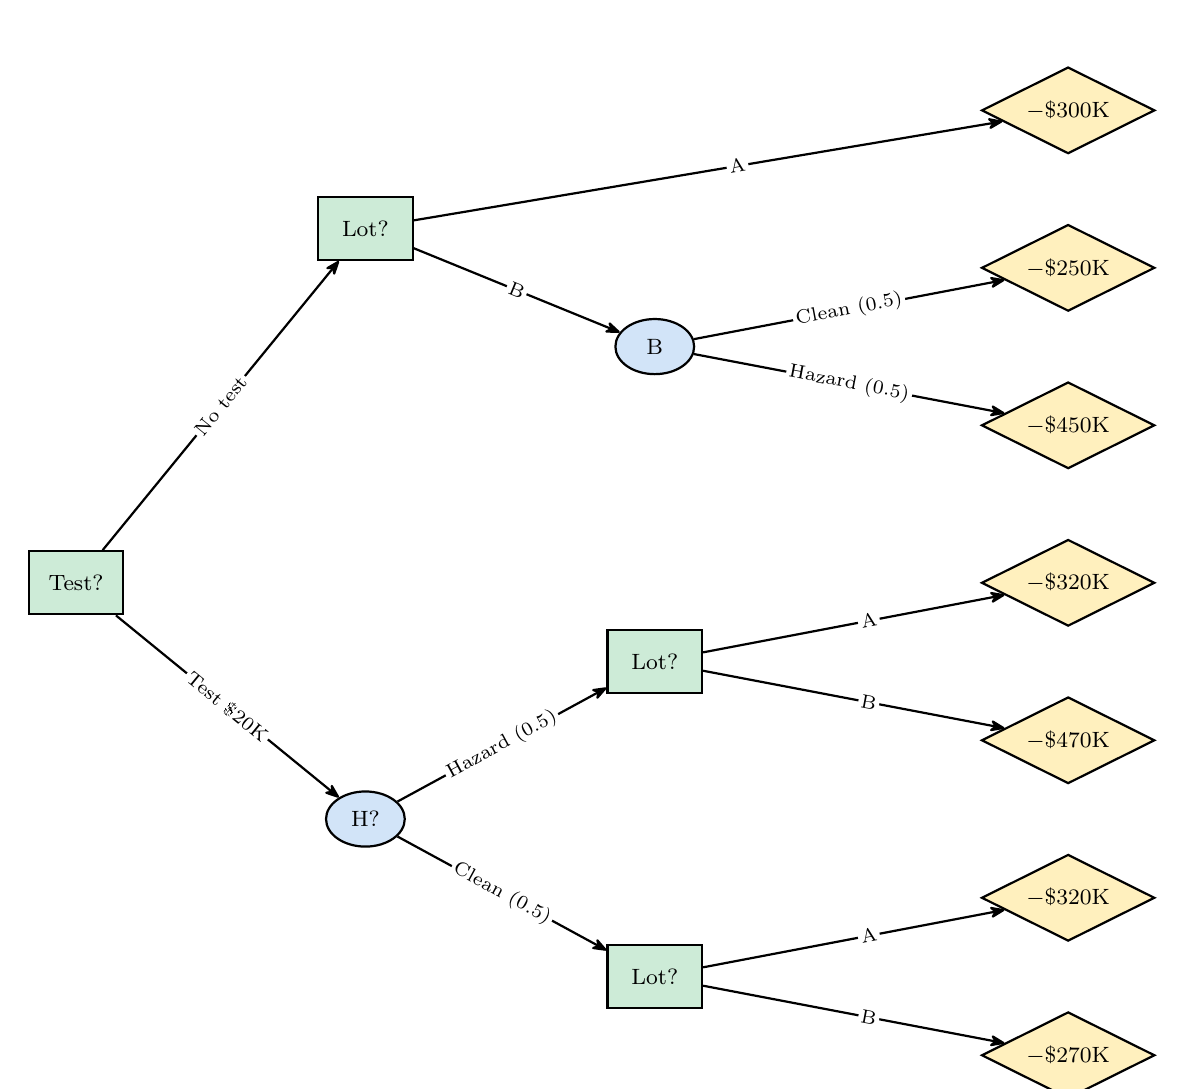
\begin{tikzpicture}[
  >={Stealth[round]},thick,x=1.05cm,y=1cm,
  decision/.style={rectangle,draw,fill=decfill,minimum width=12mm,minimum height=8mm,thick,inner sep=2pt,font=\footnotesize},
  chance/.style={ellipse,draw,fill=chancefill,minimum width=10mm,minimum height=7mm,thick,inner sep=1pt,font=\footnotesize},
  utility/.style={diamond,draw,fill=utilfill,minimum width=22mm,minimum height=11mm,thick,inner sep=-2pt,aspect=1.9,font=\footnotesize},
  every edge/.style={draw,->,thick},
  elabel/.style={font=\scriptsize,fill=white,inner sep=1pt}
]
  % --- Internal nodes (decisions and chance) ---
  \node[decision] (D0) at (0, 0)     {Test?};
  \node[decision] (D1) at (3.5, 4.5) {Lot?};
  \node[chance]   (C0) at (3.5,-3)   {H?};
  \node[chance]   (C1) at (7,  3)    {B};
  \node[decision] (DH) at (7, -1)    {Lot?};
  \node[decision] (DC) at (7, -5)    {Lot?};

  % --- Terminal utility nodes (7 leaves), evenly spaced at x=12 ---
  \node[utility] (T1A)  at (12,  6) {$-\$300$K};
  \node[utility] (T1Bc) at (12,  4) {$-\$250$K};
  \node[utility] (T1Bh) at (12,  2) {$-\$450$K};
  \node[utility] (T2A)  at (12,  0) {$-\$320$K};
  \node[utility] (T2B)  at (12, -2) {$-\$470$K};
  \node[utility] (T3A)  at (12, -4) {$-\$320$K};
  \node[utility] (T3B)  at (12, -6) {$-\$270$K};

  % --- Edges from D0 (top-level decision) ---
  \draw[->] (D0) -- (D1) node[midway,sloped,elabel]{No test};
  \draw[->] (D0) -- (C0) node[midway,sloped,elabel]{Test \$20K};

  % --- Edges from D1 (no-test lot choice) ---
  \draw[->] (D1) -- (T1A) node[midway,sloped,elabel,pos=0.55]{A};
  \draw[->] (D1) -- (C1)  node[midway,sloped,elabel]{B};

  % --- Edges from C1 (no-test, B chance) ---
  \draw[->] (C1) -- (T1Bc) node[midway,sloped,elabel,pos=0.5]{Clean (0.5)};
  \draw[->] (C1) -- (T1Bh) node[midway,sloped,elabel,pos=0.5]{Hazard (0.5)};

  % --- Edges from C0 (test result chance) ---
  \draw[->] (C0) -- (DH) node[midway,sloped,elabel]{Hazard (0.5)};
  \draw[->] (C0) -- (DC) node[midway,sloped,elabel]{Clean (0.5)};

  % --- Edges from DH (post-test, hazardous) ---
  \draw[->] (DH) -- (T2A) node[midway,sloped,elabel,pos=0.55]{A};
  \draw[->] (DH) -- (T2B) node[midway,sloped,elabel,pos=0.55]{B};

  % --- Edges from DC (post-test, clean) ---
  \draw[->] (DC) -- (T3A) node[midway,sloped,elabel,pos=0.55]{A};
  \draw[->] (DC) -- (T3B) node[midway,sloped,elabel,pos=0.55]{B};
\end{tikzpicture}}
\end{center}

\textbf{Reading the tree level by level.}
\begin{itemize}[leftmargin=1.5em,itemsep=2pt]
  \item \textbf{Root (\emph{Test?}).} The client first decides whether to hire the testing firm. The two outgoing edges are labeled ``No test'' and ``Test \$20K''.
  \item \textbf{No-test branch (top half).} The client makes the lot decision (\emph{Lot?}) using only the prior. Choosing Lot~A is deterministic at $-\$300$K. Choosing Lot~B opens a chance node $B$, where the lot turns out Clean with probability $0.5$ (cost $-\$250$K) or Hazardous with probability $0.5$ (cost $-\$250$K $-$ $\$200$K cleanup $= -\$450$K).
  \item \textbf{Test branch (bottom half).} The \$20{,}000 fee is paid up front. The chance node $H?$ then reveals \emph{with certainty} whether Lot~B is hazardous (prior $0.5$). After observing the result, the client makes an informed lot decision. The four post-test terminals all include the \$20{,}000 fee:
  \begin{itemize}[leftmargin=1.4em,itemsep=0pt]
    \item Hazardous $\to$ A: $-\$20$K $-$ $\$300$K $= -\$320$K.
    \item Hazardous $\to$ B: $-\$20$K $-$ $\$250$K $-$ $\$200$K $= -\$470$K.
    \item Clean $\to$ A: $-\$20$K $-$ $\$300$K $= -\$320$K.
    \item Clean $\to$ B: $-\$20$K $-$ $\$250$K $= -\$270$K.
  \end{itemize}
\end{itemize}
The tree has seven distinct leaves spanning every possible outcome; backward induction in part~(b) collapses these seven payoffs into a single optimal policy.

\subsection*{(b) Optimal policy via the Expected Utility Algorithm \hfill [5 pts]}

We solve by backward induction (the Expected Utility Algorithm from Lecture~4): compute expected payoffs at chance nodes by averaging, and choose the maximizer at decision nodes.

\textbf{No-test branch.} At the chance node under ``Lot B'':
\[
  \EE[\text{cost} \mid B,\,\text{no test}] = 0.5(-450\text{K}) + 0.5(-250\text{K}) = -350\text{K}.
\]
At the ``Lot?'' decision under no-test:
\[
  \max\{-300\text{K},\ -350\text{K}\} = -300\text{K} \implies \text{choose Lot A}.
\]

\textbf{Test branch.} At the ``Lot?'' decision under hazardous result:
\[
  \max\{-320\text{K},\ -470\text{K}\} = -320\text{K} \implies \text{choose Lot A}.
\]
At the ``Lot?'' decision under clean result:
\[
  \max\{-320\text{K},\ -270\text{K}\} = -270\text{K} \implies \text{choose Lot B}.
\]
Folding back at the chance node ``Hazardous?'':
\[
  \EE[\text{cost} \mid \text{test}] = 0.5(-320\text{K}) + 0.5(-270\text{K}) = -295\text{K}.
\]

\textbf{Top-level decision.}
\[
  \max\{-300\text{K},\ -295\text{K}\} = -295\text{K} \implies \text{Test}.
\]

\textbf{Optimal policy.} \emph{Hire the testing firm. If the test reports hazardous, buy Lot~A; if it reports clean, buy Lot~B.} Expected total cost is \$295{,}000, a saving of \$5{,}000 over the best no-test option (buying Lot~A outright at \$300{,}000).

\subsection*{(c) Maximum willingness to pay for the consultant \hfill [5 pts]}

Let $C$ denote the testing fee. With testing at fee $C$, the optimal post-test policy is: buy A if hazardous, buy B if clean. Expected cost:
\[
  \EE[\text{cost} \mid \text{test fee }C] = 0.5\,(-C - 300\text{K}) + 0.5\,(-C - 250\text{K}) = -C - 275\text{K}.
\]
Without testing, the optimal action is to buy Lot~A at \$300{,}000 (expected cost $-\$300\text{K}$). The client is indifferent when
\[
  -C - 275\text{K} = -300\text{K} \;\;\Longleftrightarrow\;\; C = 25\text{K}.
\]

\textbf{Maximum willingness to pay: \$25{,}000.} Above this fee the test is no longer worth it; below it (e.g., the actual fee of \$20{,}000) the test is strictly preferred.

%=======================================================================
\section*{Problem 2: Medical Testing Influence Diagram \hfill [20 pts]}
%=======================================================================

\textbf{Restated.} A medical testing company is deciding whether to launch a new diagnostic test. The model has three nodes:
\begin{itemize}[leftmargin=1.5em,itemsep=1pt]
  \item \textbf{Test Accuracy ($A$)}: chance node with $\Prb(A=\text{High}) = 0.7$, $\Prb(A=\text{Low}) = 0.3$.
  \item \textbf{Market Acceptance ($M$)}: chance node depending on $A$, with
  \[
    \Prb(M = \text{High} \mid A = \text{High}) = 0.8, \qquad \Prb(M = \text{High} \mid A = \text{Low}) = 0.3.
  \]
  \item \textbf{Profit ($P$)}: utility (value) node depending on $M$, with $P(M=\text{High}) = \$500{,}000$ and $P(M=\text{Low}) = \$100{,}000$.
\end{itemize}

\subsection*{(a) Influence diagram \hfill [10 pts]}

Following the conventions from Lecture~4 (chance node = ellipse, value/utility node = diamond), the influence diagram has the structure $A \to M \to P$. The single-letter symbols sit \emph{inside} the shapes, and the descriptive role of each node is written immediately below it:

\begin{center}
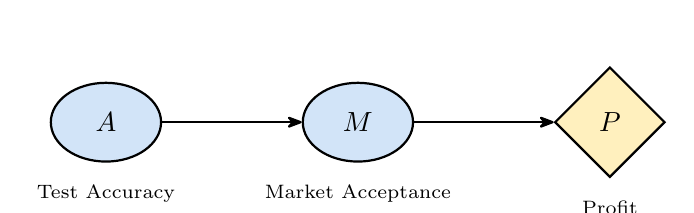
\begin{tikzpicture}[>={Stealth[round]},thick,
  chance/.style={ellipse,draw,fill=chancefill,minimum width=14mm,minimum height=10mm,thick,inner sep=1pt},
  utility/.style={diamond,draw,fill=utilfill,minimum width=14mm,minimum height=14mm,thick,inner sep=-2pt,aspect=1}]
  \node[chance]  (A) at (0, 0) {$A$};
  \node[chance]  (M) at (3.2, 0) {$M$};
  \node[utility] (P) at (6.4, 0) {$P$};
  \node[below=1.5mm of A,font=\scriptsize] {Test Accuracy};
  \node[below=1.5mm of M,font=\scriptsize] {Market Acceptance};
  \node[below=1.5mm of P,font=\scriptsize] {Profit};
  \draw[->] (A) -- (M);
  \draw[->] (M) -- (P);
\end{tikzpicture}
\end{center}

\textbf{What each piece of the diagram says.}
\begin{itemize}[leftmargin=1.5em,itemsep=1pt]
  \item Both $A$ and $M$ are \emph{chance} nodes (ellipses), representing random variables that the decision-maker observes only as outcomes, not as direct inputs.
  \item $P$ is a \emph{value} node (diamond), encoding the deterministic profit \$$500$K or \$$100$K that follows from the realized market state.
  \item The arc $A \to M$ encodes the conditional dependence of market acceptance on test accuracy: $\Prb(M \mid A)$ is given in the problem statement.
  \item The arc $M \to P$ says profit depends only on the realized market acceptance, with the deterministic mapping $P(\text{High}) = 500$K, $P(\text{Low}) = 100$K.
  \item There is \emph{no decision node} in this diagram because the question fixes the action as ``launch'' and asks only for the expected profit \emph{given} that the test is launched.
\end{itemize}

The joint factorizes via the Bayesian-network chain rule (Lecture~2):
\[
  \Prb(A, M) = \Prb(A)\,\Prb(M \mid A), \qquad \EE[P] = \sum_{m} P(m)\,\Prb(M = m).
\]

\subsection*{(b) Expected profit \hfill [10 pts]}

\textbf{Step 1: marginalize $A$ to obtain $\Prb(M = \text{High})$ via total probability.}
\begin{align*}
  \Prb(M = \text{High})
  &= \Prb(M{=}\text{H} \mid A{=}\text{H})\,\Prb(A{=}\text{H}) \\
  &\quad + \Prb(M{=}\text{H} \mid A{=}\text{L})\,\Prb(A{=}\text{L}) \\
  &= 0.8 \cdot 0.7 + 0.3 \cdot 0.3 \\
  &= 0.56 + 0.09 \;=\; 0.65.
\end{align*}
Therefore $\Prb(M = \text{Low}) = 1 - 0.65 = 0.35$.

\textbf{Step 2: compute the expected profit by averaging over $M$.}
\begin{align*}
  \EE[P] &= \Prb(M=\text{High}) \cdot \$500\text{K} + \Prb(M=\text{Low}) \cdot \$100\text{K} \\
         &= 0.65 \cdot 500\text{K} + 0.35 \cdot 100\text{K} \\
         &= 325\text{K} + 35\text{K} \;=\; \boxed{\$360{,}000}.
\end{align*}

The expected profit of launching the diagnostic test is \textbf{\$360{,}000}. Note this is the unconditional expectation, marginalizing over both the unknown accuracy and the market response.

%=======================================================================
\section*{Problem 3: Parking MDP \hfill [20 pts]}
%=======================================================================

\textbf{Restated.} Each school day you choose where to park your car: on the street in one space, on the street straddling two spaces, or in the garage. The relevant statistics are:

\begin{center}
\begin{tabular}{lccc}
\toprule
& \textbf{1 space} & \textbf{2 spaces} & \textbf{Garage} \\
\midrule
Probability of dent (per day) & $1/10$ & $1/50$ & $0$ \\
Probability of \$15 ticket & $0$ & $3/10$ & $0$ \\
Direct parking fee & \$0 & \$0 & \$5 \\
\bottomrule
\end{tabular}
\end{center}

If your car is dented, you may either \emph{repair} it (\$50 in repair fees and cab fares, car out of service for the day) or \emph{drive it dented} (loss of value/pride of \$9 per school day). The objective is to minimize long-run expected average cost per school day.

We follow the modeling pattern from Lecture~5: identify the time horizon, states, actions, transitions, rewards, and discount factor.

\subsection*{Time horizon}

Decisions are made daily, every school day. Since the problem is stated in terms of long-run average cost, we take the horizon to be infinite: $\mathcal{T} = \{1, 2, 3, \ldots\}$.

\subsection*{States}

The relevant condition that affects today's decisions is whether the car is currently dented:
\[
  s_t \in S = \{N, D\}, \qquad N = \text{not dented},\ D = \text{dented}.
\]

\subsection*{Actions}

When the car is \emph{not dented} ($s = N$), the only choice is where to park:
\[
  A(N) = \{P_1, P_2, P_G\},
\]
where $P_1$ = park in 1 space, $P_2$ = straddle 2 spaces, $P_G$ = park in the garage.

When the car is \emph{dented} ($s = D$), the action set adds the repair option:
\[
  A(D) = \{R, P_1', P_2', P_G'\},
\]
where $R$ = repair (car out of service that day) and the primed actions $P_1', P_2', P_G'$ mean ``drive the car \emph{dented} and park in the indicated location.''

\subsection*{Transition probabilities}

The car can become dented only when not currently dented; once dented it remains dented until repaired (we treat ``dented'' as a binary condition). Repairing returns the car to the not-dented state with probability one.

\textbf{From $s = N$:}
\begin{align*}
  p(N \mid N, P_1) &= 9/10, & p(D \mid N, P_1) &= 1/10, \\
  p(N \mid N, P_2) &= 49/50, & p(D \mid N, P_2) &= 1/50, \\
  p(N \mid N, P_G) &= 1, & p(D \mid N, P_G) &= 0.
\end{align*}

\textbf{From $s = D$:}
\begin{align*}
  p(N \mid D, R) &= 1, & p(D \mid D, R) &= 0, \\
  p(D \mid D, P_1') &= 1, & p(D \mid D, P_2') &= 1, & p(D \mid D, P_G') &= 1.
\end{align*}
(After repair the car is fresh; if you drive dented, the car stays dented.)

\subsection*{Rewards (negative costs)}

Rewards are the negative of expected daily cost incurred under the chosen action. From $s = N$:
\begin{align*}
  r(N, P_1) &= -\$0 = 0, \\
  r(N, P_2) &= -\EE[\text{ticket}] = -\tfrac{3}{10}\cdot\$15 = -\$4.50, \\
  r(N, P_G) &= -\$5.
\end{align*}
From $s = D$:
\begin{align*}
  r(D, R) &= -\$50 \quad \text{(repair fees and cab fares; no parking choice that day)}, \\
  r(D, P_1') &= -\$9 \quad \text{(drive dented; no street ticket since 1-space)}, \\
  r(D, P_2') &= -\$9 - \tfrac{3}{10}\cdot\$15 = -\$13.50, \\
  r(D, P_G') &= -\$9 - \$5 = -\$14.
\end{align*}

\subsection*{Discount factor}

The objective is the \emph{long-run expected average cost}, an average-reward MDP, so a discount factor is not strictly needed. Equivalently we may use $\lambda = 1$ in the formulation; or, if a discounted formulation is preferred for tractability, take $\lambda$ slightly below~$1$.

\subsection*{Summary}

The MDP tuple is
\[
  \big(\mathcal{T} = \{1, 2, \ldots\},\ S = \{N, D\},\ A,\ p,\ r,\ \lambda\big),
\]
with the components above. The optimal policy will trade off the small expected ticket cost on 2 spaces (\$4.50/day) against the dent-protection benefit; once dented, it will weigh the per-day pride cost (\$9) against the one-time repair cost (\$50). Solving for the optimal policy is left to the algorithms of Lectures~6--7 (backward induction or value iteration).

%=======================================================================
\section*{Problem 4: 3-Piece Tic-Tac-Toe MDP \hfill [20 pts]}
%=======================================================================

\textbf{Restated.} Two players play a turn-taking game on a $3 \times 3$ board, each holding three pieces. Each turn, a player either (i) places one of their off-board pieces into a free slot, or (ii) if all three of their pieces are already on the board, takes one of their pieces off the board and places it elsewhere on a free slot. The objective is to align all three of one's pieces in a row, column, or diagonal.

We model this as an MDP from \emph{our} player's point of view, treating the opponent's behavior as part of the (stochastic) environment.

\subsection*{Time horizon}

The game is sequential and could in principle continue indefinitely (since pieces can be relocated), so we take an infinite horizon $\mathcal{T} = \{1, 2, \ldots\}$ with absorbing terminal states (win/loss/draw). For tractability we typically also use a discount factor $\lambda \in (0, 1)$.

\subsection*{States}

A state $s_t$ is a complete board configuration as observed by our player when it is our turn to move:
\[
  s_t \in S \subseteq \{\text{empty},\ \text{me},\ \text{opp}\}^9.
\]
Each of the nine cells is labeled with one of three symbols. Valid configurations have at most three of our pieces and at most three of the opponent's pieces on the board. Among these we mark certain configurations as \emph{terminal}:
\begin{itemize}[leftmargin=1.5em,itemsep=1pt]
  \item $S_{\text{win}}$: configurations where our three pieces form a row, column, or diagonal.
  \item $S_{\text{lose}}$: configurations where the opponent's three pieces form a row, column, or diagonal.
  \item $S_{\text{draw}}$: configurations where neither side can win (rare in this movement variant; usually omitted).
\end{itemize}
We do not include ``whose turn'' in the state because the MDP is defined to capture only \emph{our} decisions: by convention, every non-terminal $s_t$ is a position in which it is our turn to move.

\subsection*{Actions}

The action set $A(s_t)$ depends on how many of our pieces are already on the board.

\textbf{Case 1: fewer than three of our pieces are on the board (placement phase).} The action is to place one off-board piece on any empty cell:
\[
  A(s_t) = \{(\text{place}, c) : c \text{ empty in } s_t\}.
\]

\textbf{Case 2: all three of our pieces are on the board (movement phase).} The action is to pick up one of our on-board pieces and re-place it on a different empty cell:
\[
  A(s_t) = \{(\text{move},\ c_{\text{from}},\ c_{\text{to}}) : c_{\text{from}} \text{ holds our piece, } c_{\text{to}} \text{ empty}\}.
\]

In terminal states $A(s_t) = \emptyset$ (game over, no further actions).

\subsection*{Transition probabilities}

A transition $s_t \xrightarrow{a_t} s_{t+1}$ in our MDP is composed of two micro-steps:

\textbf{Micro-step 1 (deterministic).} Apply our move $a_t$ to $s_t$; this gives an intermediate configuration $s_t' = \text{Apply}(s_t, a_t)$.

\textbf{Micro-step 2 (stochastic).} The opponent now moves. Let $\pi_{\text{opp}}(\cdot \mid s_t')$ be the opponent's (possibly randomized) policy, which we treat as part of the environment. Then
\[
  p_t(s_{t+1} \mid s_t, a_t) = \sum_{a'} \mathbf{1}\{s_{t+1} = \text{Apply}(s_t', a')\}\;\pi_{\text{opp}}(a' \mid s_t').
\]
Two natural choices of opponent model: (i) \emph{uniform random} opponent, $\pi_{\text{opp}}$ uniform on legal moves --- the simplest baseline; (ii) \emph{minimax} opponent, $\pi_{\text{opp}}$ deterministic best-response. The MDP framework accommodates either.

\textbf{Special cases.} If $s_t'$ is already terminal (we just won), the game ends and there is no opponent move; transition into the terminal absorbing state is deterministic. Similarly if the opponent's move makes the resulting state terminal (we lose), the chain absorbs there.

\subsection*{Rewards}

A standard zero-sum game reward gives credit only at the end:
\[
  r_t(s_t, a_t, s_{t+1}) = \begin{cases}
    +1, & s_{t+1} \in S_{\text{win}} \quad \text{(we win)}, \\
    -1, & s_{t+1} \in S_{\text{lose}} \quad \text{(we lose)}, \\
    0,  & \text{otherwise}.
  \end{cases}
\]
Intermediate rewards may also be added (e.g., bonuses for two-in-a-row threats), but the cleanest formulation uses only terminal rewards. In absorbing terminal states, all rewards are $0$ thereafter.

\subsection*{Discount factor}

A discount factor $\lambda \in (0, 1)$ captures the preference for winning sooner rather than later (since the game can in principle continue indefinitely under the movement phase). A typical choice is $\lambda \in [0.95, 0.99]$. Without discounting ($\lambda = 1$) the value function is still well-defined provided the game terminates almost surely.

\subsection*{Summary}

The MDP tuple is
\[
  \big(\mathcal{T} = \{1,2,\ldots\},\ S,\ A,\ p,\ r,\ \lambda\big),
\]
with $S$ the (finite, large) set of board configurations, $A(s)$ the placement-or-movement action set, $p$ governed by our deterministic move plus the opponent's stochastic response, and $r$ giving $\pm 1$ at terminal states. Solving this MDP exactly is computationally feasible because the state space is finite (though large); methods like value iteration and reinforcement-learning self-play apply directly.

%=======================================================================
\section*{Problem 5: Term Project Preliminary Description \hfill [20 pts]}
%=======================================================================

\textbf{Project title.} \emph{Regime-Switching Asset Allocation via a Partially Observable Markov Decision Process.}

\textbf{Team.} Dario Blanco Morales, Even Hogberget, Kyle David Ledda-Lewaren, Taka Khoo.

\subsection*{(a) Modeling framework \hfill [5 pts]}

We model the problem as a \textbf{Partially Observable Markov Decision Process (POMDP)} solved approximately via the \textbf{QMDP} approximation. We \emph{do not} use a decision tree, an influence diagram, or a fully-observable MDP, and the reasons are concrete:

\begin{itemize}[leftmargin=1.5em,itemsep=2pt]
  \item \textbf{Decision trees} unfold every random outcome explicitly. With monthly rebalancing over decades and a small but nontrivial action set, the number of paths is astronomical and the tree representation is impractical.
  \item \textbf{Influence diagrams} model a single-stage or fixed-stage decision under uncertainty. They do not capture the recursive, dynamic decision-making implied by repeated rebalancing.
  \item \textbf{A standard MDP} would require us to know the current market regime --- but \emph{the regime is not directly observable}. We see noisy proxies (VIX, term spread, high-yield OAS), not the latent state. The whole point of a Hidden Markov Model in our pipeline is to estimate a posterior \emph{belief} over the regime; using that belief as the input to a control problem is exactly what a POMDP formalizes.
  \item \textbf{POMDP} is the natural fit: a Markov chain over latent regimes, observations that depend on the current regime via the HMM emission distributions, and discrete portfolio actions with rewards driven by realized returns and a utility function. Because exact POMDP solution is generally intractable, we will use the QMDP approximation $Q_{\text{QMDP}}(b,a) = \sum_s b(s)\,Q^*_{\text{MDP}}(s,a)$, which leverages a fully-observable MDP solution combined with the current belief.
\end{itemize}

\subsection*{(b) Elements of the model \hfill [5 pts]}

We list the POMDP tuple $(\mathcal{T}, S, A, T, \Omega, O, R, \lambda)$ explicitly.

\textbf{Time horizon $\mathcal{T}$.} Monthly decision epochs over the available data window 1990--present, $T \approx 420$ epochs in backtesting. For policy computation we treat the problem as effectively infinite-horizon discounted ($\lambda$ below).

\textbf{States $S$ (latent regimes).} The latent macro-financial regimes we infer from a Gaussian HMM. Two-state baseline:
\[
  S = \{\text{Expansion},\ \text{Stress}\}.
\]
We will also evaluate a three-state extension $S = \{\text{Expansion},\ \text{Transition},\ \text{Stress}\}$ via BIC and out-of-sample log-likelihood.

\textbf{Actions $A$ (portfolio weights).} A discrete grid of stock--bond allocations:
\[
  A = \big\{(w_S, w_B) \,:\, w_S + w_B = 1,\ w_S \in \{0, 0.25, 0.5, 0.75, 1\}\big\}.
\]
Discretization keeps the QMDP value-iteration table small while spanning typical institutional risk profiles.

\textbf{Transition function $T(s' \mid s)$.} The HMM transition matrix estimated by Baum--Welch on the observation series. The action does not affect the regime transitions (the market is exogenous to our portfolio choice).

\textbf{Observations $\Omega$ and observation function $O(o \mid s)$.} Observations are continuous vectors
\[
  o_t = (\text{VIX}_t,\ \text{T10Y3M}_t,\ \text{HY OAS}_t) \in \R^3.
\]
The observation function is the per-state Gaussian emission of the HMM:
\[
  O(o \mid s) \;=\; \mathcal{N}\!\big(o ;\; \mu_s,\ \Sigma_s\big), \quad s \in S,
\]
with $(\mu_s, \Sigma_s)$ estimated jointly with the transition matrix.

\textbf{Belief state $b_t$.} Posterior over regimes given observation history,
\[
  b_t(s) \;=\; \Prb(s_t = s \mid o_{1:t},\,a_{1:t-1}),
\]
updated by the standard Bayes filter (forward algorithm) using $T$ and $O$.

\textbf{Reward $R(s, a)$.} Single-period utility of the (random) portfolio return less proportional transaction costs:
\[
  R_t(s, a) \;=\; \EE\!\left[ U\!\left(a^\top R_t^{\text{asset}}\right) \;\middle|\; s_t = s \right] \;-\; c \cdot \|a_t - a_{t-1}\|_1,
\]
where $R_t^{\text{asset}} = (R_t^{\text{stock}}, R_t^{\text{bond}})^\top$ are realized asset returns, $U$ is a concave utility function (we use log utility or CRRA), and $c$ models a 5~bps cost per side per unit of weight changed.

\textbf{Discount factor $\lambda$.} $\lambda = 0.99$ at monthly resolution, reflecting a roughly 8-year effective planning horizon (since $1/(1-\lambda) \approx 100$ months).

\subsection*{(c) Objective and value function \hfill [10 pts]}

\textbf{Decision-maker's objective.} Maximize the expected discounted sum of realized utilities of portfolio returns, net of transaction costs, subject to information available at each rebalance:
\[
  \pi^* \;\in\; \argmax_{\pi}\ \EE_{\pi}\!\left[\, \sum_{t=1}^{T} \lambda^{t-1}\, R_t\bigl(s_t, \pi(b_t)\bigr) \,\right].
\]
The maximization is over policies that map belief states $b_t$ to actions $\pi(b_t) \in A$.

\textbf{Utility function.} Log utility (constant relative risk aversion with $\gamma = 1$) is our default,
\[
  U(R_p) \;=\; \log\!\big(1 + R_p\big),
\]
where $R_p = a^\top R^{\text{asset}}$ is the portfolio return. We will report sensitivity to the more general CRRA family
\[
  U_\gamma(R_p) \;=\; \frac{(1 + R_p)^{1-\gamma}}{1 - \gamma}, \qquad \gamma \in \{2, 5\},
\]
to demonstrate robustness of the regime-aware policy across risk aversions.

\textbf{Value function (Bellman equation in belief space).} The optimal value function over beliefs satisfies
\[
  V^*(b) \;=\; \max_{a \in A}\!\left\{\, R(b, a) \;+\; \lambda \sum_{o \in \Omega} \Prb(o \mid b, a)\, V^*\!\big(b' \mid b, a, o\big) \,\right\},
\]
with $R(b, a) = \sum_{s} b(s)\, R(s, a)$ and the next belief $b' \mid b, a, o$ obtained by Bayes filtering.

Because exact solution of the belief-space Bellman equation is intractable for general POMDPs, we adopt the \textbf{QMDP approximation} (Littman, Cassandra, Kaelbling, 1995):
\begin{align*}
  Q_{\text{QMDP}}(b, a) &= \sum_{s \in S} b(s)\, Q^*_{\text{MDP}}(s, a), \\
  \pi_{\text{QMDP}}(b)  &= \argmax_{a \in A}\, Q_{\text{QMDP}}(b, a),
\end{align*}
where $Q^*_{\text{MDP}}(s, a)$ is the optimal action-value function of the underlying \emph{fully-observable} MDP --- itself solved by standard value iteration. Intuitively, QMDP weights the per-regime $Q$-values by our posterior belief over the regime; it is exact in the fully-observable limit and a sensible heuristic when uncertainty is moderate.

\textbf{Comparator policies.} We will also evaluate (i) a myopic one-step-lookahead policy $\pi_{\text{myopic}}(b) = \argmax_a R(b, a)$ that ignores future evolution of beliefs, and (ii) the static 60/40 benchmark $\pi_{\text{static}}(b) = (0.6, 0.4)$ for all $b$. Out-of-sample backtests will compare CAGR, volatility, Sharpe ratio, maximum drawdown, and Calmar ratio across the three policies, with sensitivity analysis over the number of regimes (2 vs.\ 3), rebalancing frequency, and transaction-cost level.

\textbf{Connection to the lecture material.} This POMDP setting fuses Lecture~2 (Bayesian inference of latent variables --- here a Bayesian filter over regimes), Lecture~3 (a Markov chain on regimes), Lecture~4 (decision-graph reasoning over multiple periods), and the Lecture~5--6 MDP machinery (sequential decisions, value functions, Bellman equations). The QMDP approximation, in turn, foreshadows the dynamic-programming and reinforcement-learning content in Parts~III--IV of the course.

\end{document}
